\documentclass[10pt,twocolumn]{article}
\usepackage{latex8}
\usepackage[letterpaper]{geometry}
\usepackage{times}
\usepackage{xurl}
\usepackage{graphicx}
\usepackage{amssymb}
\usepackage{float}
\usepackage{hyperref}
\usepackage{cleveref}
\usepackage{booktabs}
\usepackage{tabularray}
\usepackage{listings}
\usepackage{inconsolata}
\usepackage{rosepine}
\usepackage{jsonlisting}
\usepackage[T1]{fontenc}

\UseTblrLibrary{booktabs}
\Crefname{lstlisting}{Listing}{Listings}
\crefname{lstlisting}{listing}{listings}

% NOTE: Limit listing line length to 40 characters (before it crosses the border)!

\newcommand{\term}[1]{%
    \emph{#1}%
}

\pagestyle{empty}

\title{
	A Framework for Automated Functional \\
	Testing of Environmental Models
}
\author{
	Aidan Bensch$^1$, Sam Allen$^1$, Lan Lin$^1$, Peter Schwartz$^2$, Dali Wang$^2$
}

\affiliation{
	\small
	$^1$Department of Computer Science,
	Ball State University,
	Muncie, IN 47306, USA \\
	\small
	\{aidan.bensch, sallen7, llin4\}@bsu.edu \\
	\small
	$^2$Environmental Sciences Division,
	Oak Ridge National Laboratory,
	Oak Ridge, TN 37831, USA \\
	\small
	\{schwartzpd, wangd\}@ornl.gov
}

\begin{document}

% Questions for Peter and Dali:
% Are we correct about existing testing for E3SM?

\maketitle

\thispagestyle{empty}

\abstract
The Energy Exascale Earth System Model (E3SM) has extensive system and 
regression testing, but it lacks automated functional testing at the subroutine level. To
address this need, we propose an extensible automated testing framework designed around the Software Package for E3SM Land Model (ELM) (SPEL). It supports 
multiple implementations for input space reduction and for tackling the test oracle problem. Using the framework, we applied change-impact analysis as well as combinatorial and 
property-based testing to \verb|LakeTemperature|, a subroutine in ELM responsible for 
simulating changes in the temperature of a lake. Our preliminary results led to further examining the code base for \verb|LakeTemperature| and SPEL for bugs, 
which demonstrates the usefulness of our testing 
framework and its value as a tool for testing other ELM modules in the future.
\endabstract

\section{Introduction}
\label{sec:introduction}

The Energy Exascale Earth System Model (E3SM) \cite{e3sm}, developed by the US 
Department of Energy, is an Earth model that aids in research pertaining to the 
climate and energy-relevant science. As with any scientific software, it is 
important to test the software for correctness and to identify edge cases. E3SM has 
been tested extensively in the past, including system and regression testing using the 
Common Infrastructure for Modeling the Earth (CIME)'s framework \cite{cime}, as 
well as scientific validation using the E3SM Diagnostics package \cite{e3sm-diag}.

% Take a look at this paragraph's end to see if that works well.

The Software Package for E3SM Land Model (SPEL) was developed to automate the generation
of standalone unit tests by analyzing the code of the E3SM Land Model (ELM) and performing 
bit-for-bit verification against a reference output \cite{spel}. SPEL's unit tests make it 
possible to run and test individual subroutines of ELM in isolation, and provide a 
NetCDF \cite{netcdf} interface for controlling \term{model constants},
and observing \term{model outputs}. For functional testing to be 
effective, various combinations of model constants need to be exercised, and 
the outputs need to be validated beyond bit-for-bit validation.

Our primary contribution in this paper is the automated testing framework we
developed to address this need, which supports multiple methods for changing model 
constants and validating model outputs through the use of {\it sampling} and {\it 
analysis} plugins. To demonstrate the use of our framework, we applied it to test
\verb|LakeTemperature|, an ELM subroutine that simulates temperature changes in lakes 
\cite{laketemperature}. We performed change-impact analysis as well as combinatorial and 
property-based testing on \verb|LakeTemperature|, allowing us to find relationships 
between model constants and model outputs, as well as verify outputs following physical laws.

This paper is organized as follows. \Cref{sec:background} details concepts and tools we 
applied in our testing of \verb|LakeTemperature|, and compares our work to similar 
projects. \Cref{sec:framework} describes the design and implementation 
of our testing framework. \Cref{sec:application} elaborates on our application of it to 
\verb|LakeTemperature|. \Cref{sec:results} provides details about the results of our case 
study. Finally, \Cref{sec:conclusion} concludes the paper and identifies directions for 
future work.

\section{Background and Related Work}
\label{sec:background}

E3SM is composed of several high-level \term{component models}. Both E3SM and its component
models have been tested previously. Scientific validation is done using the E3SM 
Diagnostics package \cite{e3sm-diag}, which compares E3SM output to real-world 
observations or output from another model. System and regression testing is performed 
using CIME's framework \cite{cime}. The E3SM Land Model (ELM), the component model 
that \verb|LakeTemperature| is a part of, uses CIME's regression tests to compare 
``baseline'' output of ELM at an earlier point in development to its current output
\cite{elm-testing}. To the best of our knowledge, there is not a framework for 
automated functional testing of subroutines (like \verb|LakeTemeperature|) in 
ELM.

When testing \verb|LakeTemperature|, we control 17 model constants, 13 of which are
floating-point or integer valued. It is computationally infeasible to
extensively test the entire input space, so we need to reduce it while still covering the 
most important cases. One approach is {\it statistical testing}, which uses probability to 
sample input values and make assertions about the reliability of the software 
\cite{statistical-cleanroom}, such as when testing embedded systems
\cite{statistical-embedded}. 
Another approach is {\it combinatorial testing}, which is 
predicated on the idea that most software failures occur due to interactions between very 
few inputs, and by testing all $t$-way combinations, results similar to that 
of exhaustive testing can be achieved with significantly fewer test cases 
\cite{combinatorial-emperical}. %It has been applied to test REST APIs 
%\cite{combinatorial-rest-apis} and analyze fairness in machine learning models 
%\cite{combinatorial-ml-fairness}.

\verb|LakeTemperature| simulates a complex physical process, so it is hard to  
determine what constitutes ``correct'' output, a challenge commonly referred to as the
\term{test oracle} problem \cite{test-oracle}. One approach to this is 
{\it metamorphic testing} \cite{metamorphic-survey}, which uses known 
relationships between combinations of inputs and outputs to validate the output, rather 
than checking for specific output values. It has been applied to hydrological models 
driven by machine learning \cite{metamorphic-ml-hydro}. %and graphics compilers 
%\cite{metamorphic-graphics}. 
Another approach is {\it property-based testing}, 
which asserts that the output demonstrates properties we know must be followed for any 
given input. It has been used to test agent-based scientific models
\cite{property-based-abs}, %and %OCaml 5's runtime system \cite{property-based-ocaml}, 
as well as EAMxx, the new C++ port of the E3SM Atmosphere Model 
\cite{eamxx}.

ELM currently has system and integration tests through CIME, but lacks functional testing
beyond the bit-for-bit unit testing provided by SPEL. Our proposed testing framework, 
built around SPEL's unit tests, aims to automate functional testing for ELM subroutines 
and support multiple testing methods.

\section{
    \texorpdfstring{\raggedright A Proposed Automated Testing \\ Framework}
    {A Proposed Automated Testing Framework}
}
\label{sec:framework}

There are a number of possible solutions to reduce the input space and to solve the test 
oracle problem, so we decided to abstract each problem into its own extensible phase of 
our testing framework. They are known as the \term{sampling} phase and the 
\term{analysis} phase. Between the two is the \term{testing} phase, where we run the unit test created by SPEL. A high-level overview of these phases can be seen in 
\Cref{fig:framework_high_level}.

\begin{figure}[ht]
    \centering
    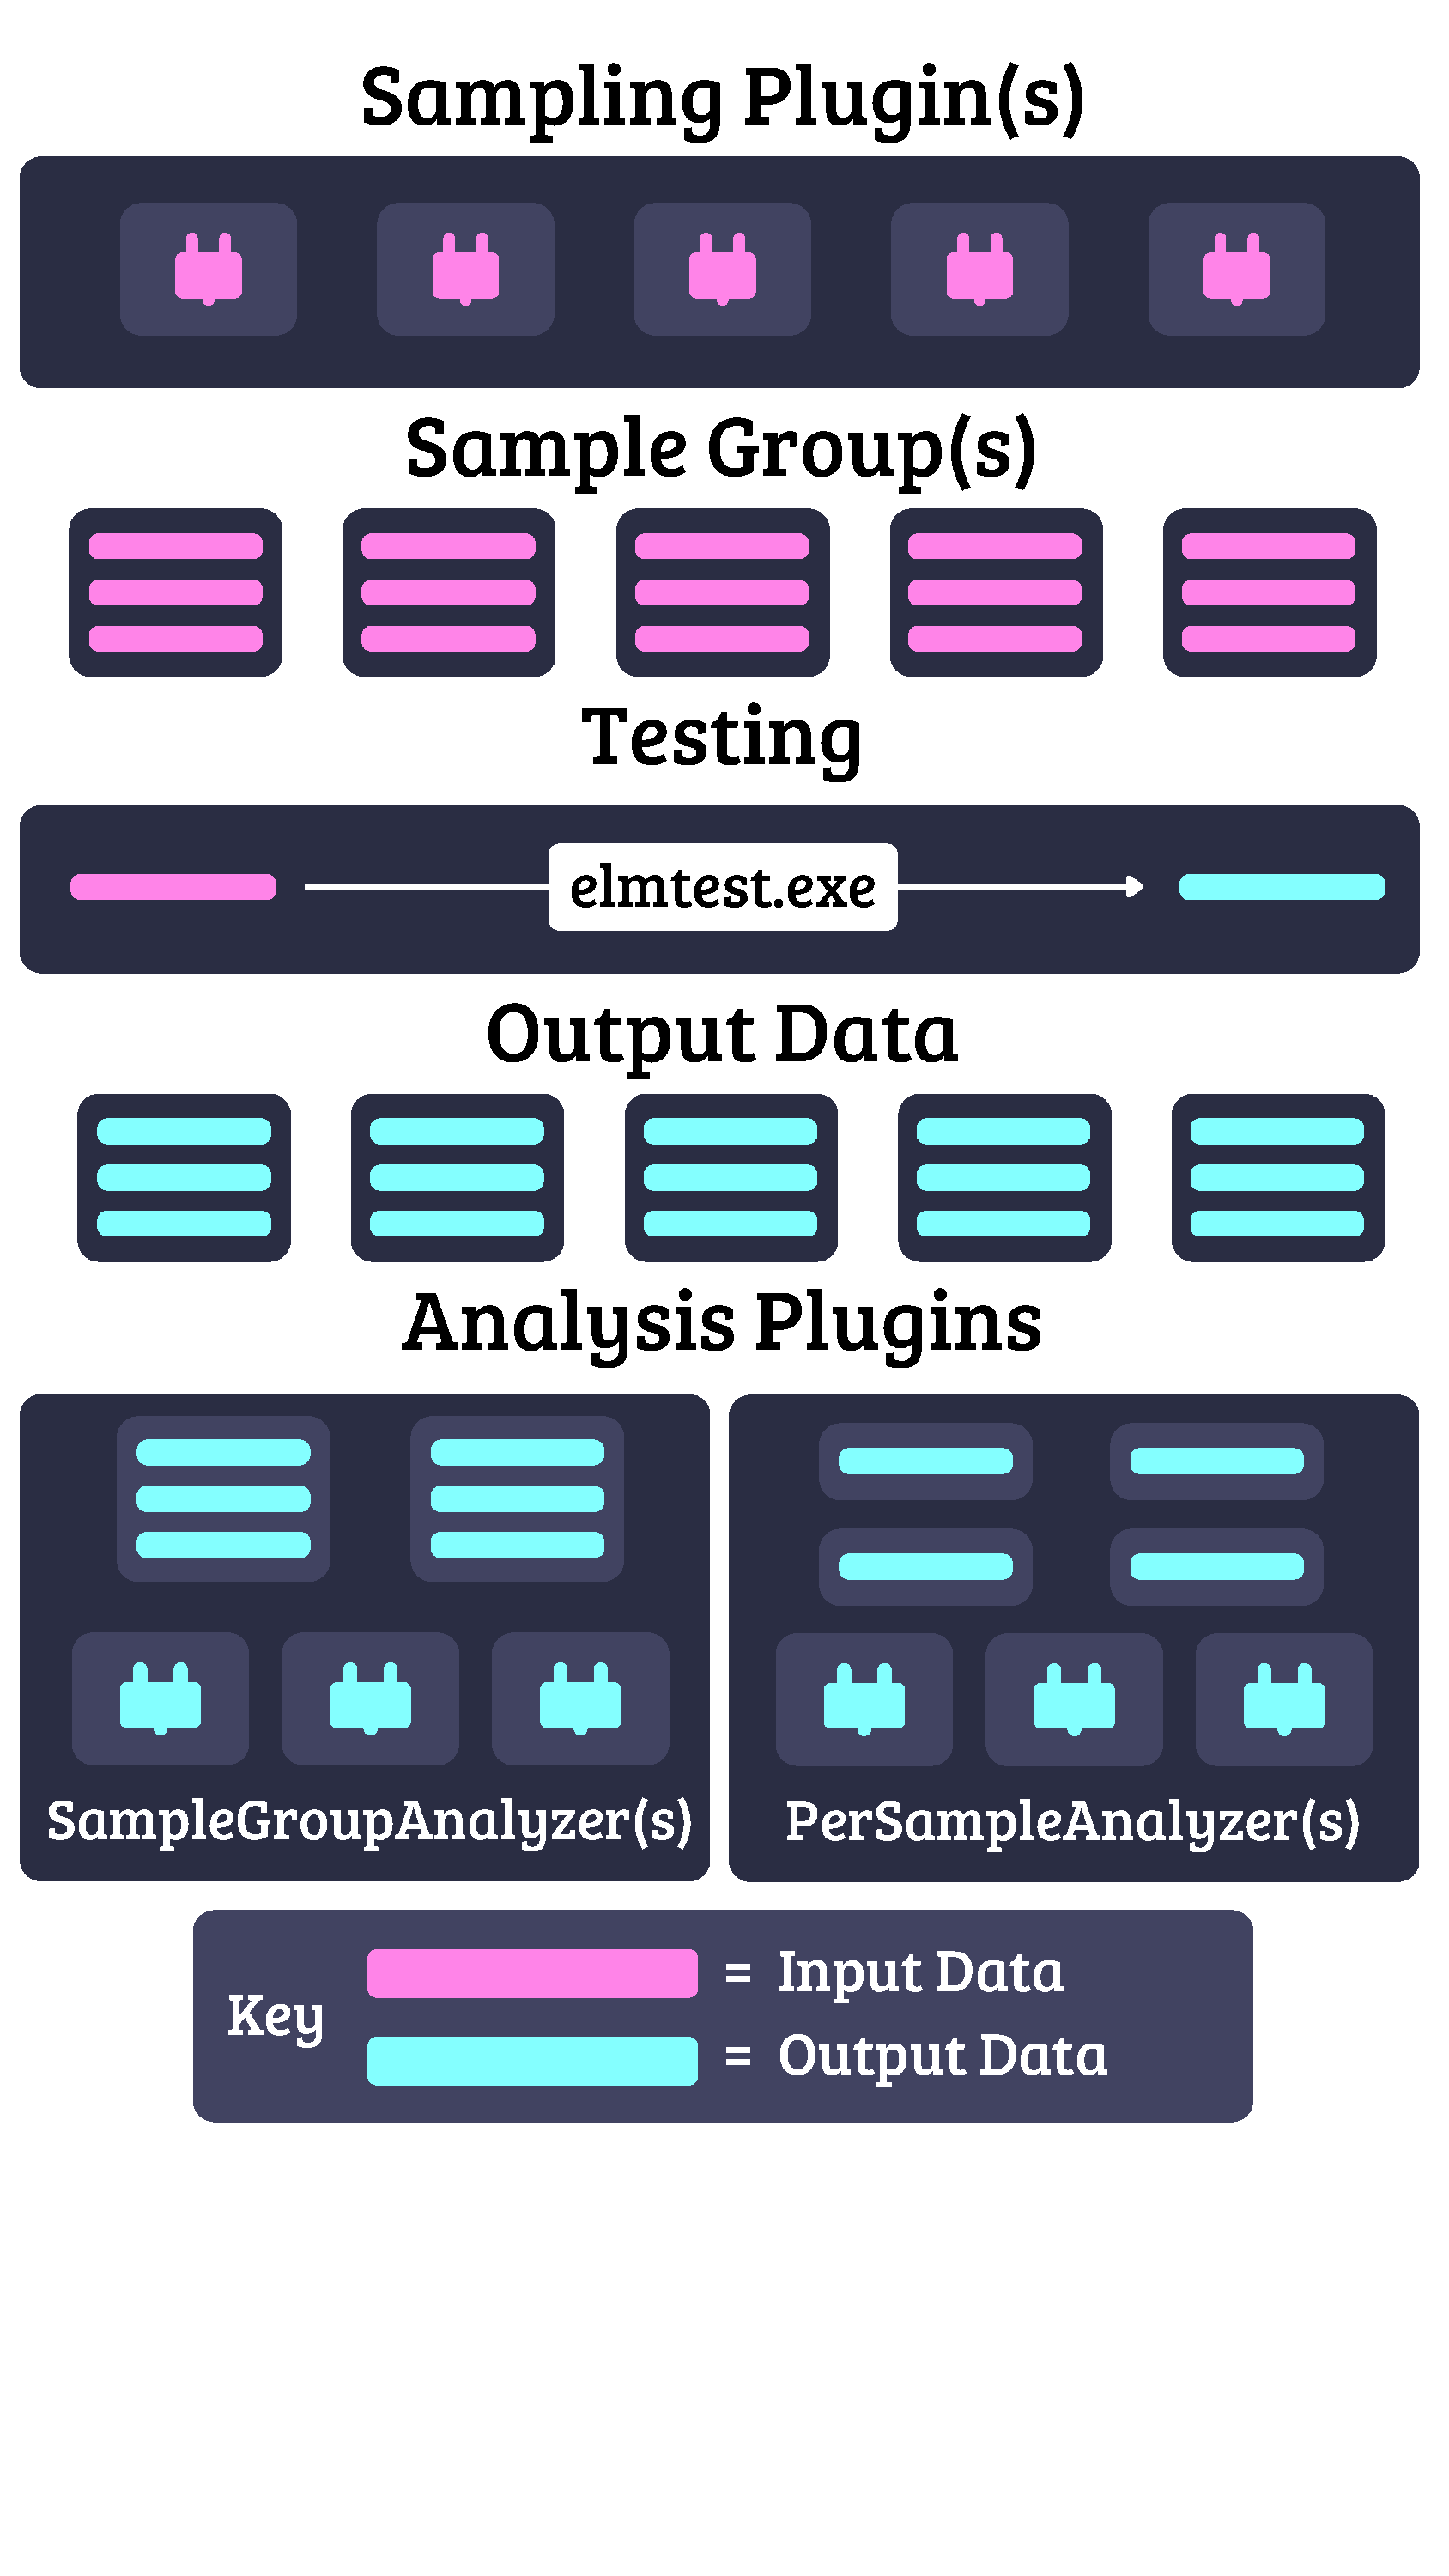
\includegraphics[width=0.85\columnwidth]{figures/testing_framework_process.pdf}
    \caption{A diagram showing a high-level overview of our testing framework}
    \label{fig:framework_high_level}
\end{figure}

SPEL allows us to create and compile a ``unit test'' for \verb|LakeTemperature|, which is 
an executable named \verb|elmtest.exe|. It exposes a NetCDF (self-describing data format
for multidimensional data \cite{netcdf}) interface for us to modify model constants and 
read model outputs. Our framework automates the process of repeatedly setting 
model constants, running \verb|elmtest.exe|, and analyzing model outputs.

The sampling phase of the framework is responsible for systematically choosing values for 
the model constants. Each \term{sampling plugin} represents a different method for 
choosing their values, and is responsible for generating {\it samples}. Each sample
contains values for the model constants, which are assigned before an individual run of 
\verb|elmtest.exe|. A JSON representation of a sample can be seen in 
\Cref{lst:json_sample}.

\begin{lstlisting}[
    language=json,
    float,
    floatplacement=ht,
    caption=JSON representation of a sample,
    label=lst:json_sample
]
{
  "betavis": 0.0,
  "cnfac": 0.5,
  "lake_no_ed": false,
  "nlevsno": 5,
  #...
}
\end{lstlisting}

Sampling plugins can also organize samples into \term{sample groups}, which allow similar 
samples to be analyzed in a shared context during the analysis phase. Each 
sampling plugin extends the \verb|Sampler| abstract class and creates at least one sample 
group. A minimal implementation is provided in \Cref{lst:sampling_plugin_example}.
\Cref{tab:sampling_plugins} details the sampling plugins we have implemented.

\begin{lstlisting}[
    language=python,
    float,
    floatplacement=ht,
    caption=Minimal implementation of a sampling plugin,
    label=lst:sampling_plugin_example
]
class MinimalSampler(Sampler):
  def get_sample_groups(self):
    samples = [
      Sample({"betavis": np.array(0.0)}),
      Sample({"betavis": np.array(0.5)}),
      Sample({"betavis": np.array(1.0)}),
    ]
    groups = {
      "group_name": SampleGroup(samples)
    }

    return groups
\end{lstlisting}

\begin{table}[tb]
    \centering
    \footnotesize
    \caption{Currently supported sampling plugins}
    \label{tab:sampling_plugins}
    \begin{tblr}{
            colspec={l X},
            width=\columnwidth
        }
        \toprule
        NetCDF Cases
        & Loads test cases from a compressed NetCDF file, each of which constitutes a
        sample group \\
        \midrule
        Order Sampling
        & Generates Order(s). Each Order reads instructions from a JSON file to
        generate samples using linear interpolation. Each Order will return one sample 
        group. \\
        \bottomrule
    \end{tblr}
\end{table}

The analysis phase processes model outputs in combination with the samples used to 
produce them in order to derive meaningful results. Analysis plugins can be used to 
implement a solution to the test oracle problem, reporting whether or not a set of output data is ``correct.'' They can also be used to filter or aggregate data into a 
useful format.

Analysis plugins extend \verb|PerSampleAnalyzer| or \verb|SampleGroupAnalyzer|.
\verb|PerSampleAnalyzer|-based plugins are run each time
\verb|elmtest.exe| finishes execution and analyze the sample with its
resulting output data. \verb|SampleGroupAnalyzer|-based plugins don't run until an entire
sample group has been tested, and they analyze outputs in the context of the group as a
whole. \Cref{lst:analysis_plugin_example} provides a minimal implementation of an 
analysis plugin.  \Cref{tab:analysis_plugins} describes the analysis plugins we have 
written.

\begin{lstlisting}[
    language=python,
    float,
    floatplacement=ht,
    caption=Minimal implementation of an analysis plugin,
    label=lst:analysis_plugin_example
]
class MinimalAnalyzer(SampleGroupAnalyzer):
  OUTPUT_NAME = "lakestate_vars__betaprime_col"
  def analyze_sample_data(
    self, sample_group,
    _reference_data, sample_data,
  ):
    total_betaprime_sum = 0.0
    for indiv_data in sample_data:
      # Data is lazy loaded from disk.
      with indiv_data:
        total_betaprime_sum += np.sum(
          indiv_data[OUTPUT_NAME]
        )

    # Optional color.
    console_out = ansi.with_ansi_color(
      str(total_betaprime_sum),
      ansi.AnsiColor.BRIGHT_BLUE,
    )
    file_out = FileSystemTree.create_from_file(
      # Can use TEMP_FILE instead to write to a
      # temp file then copy it over.
      ".txt", FileReadType.IN_MEMORY,
      # BinaryIO can be used for binary files.
      io.StringIO(str(total_betaprime_sum)),
    )

    return console_out, file_out
\end{lstlisting}

\begin{lstlisting}[
    language=python,
    float,
    floatplacement=ht,
    caption=An example order interpolating betavis between 0.0 and 1.0,
    label=lst:example_order
]
{
  "samples": 11,
  "ranges": {
    "betavis": ["0.0", "1.0"]
  }
}
\end{lstlisting}

\begin{table*}[tb]
    \centering
    \footnotesize
    \caption{Currently supported analysis plugins}
    \label{tab:analysis_plugins}
    \begin{tblr}{
            colspec={l l X[4]},
            width=\textwidth
        }
        \toprule
        \SetCell[r=2]{}
        \texttt{PerSampleAnalyzer}
        & Differences 
        & Pinpoints the location and magnitude of differences between the reference data and the current sample's data \\
        \midrule
        & Fault Finding 
        & Uses \term{check} functions defined by the plugin to make assertions about values in the sample data \\ 
        \midrule
        \SetCell[r=2]{}
        \texttt{SampleGroupAnalyzer}
        & Change Detection
        & Identifies which model inputs and outputs differ from the reference \\
        \midrule
        & NetCDF4 Output
        & Stores each sample group as an individual NetCDF file \\ 
        \bottomrule
    \end{tblr}
\end{table*}

\section{Application to \texttt{LakeTemperature}}
\label{sec:application}

\verb|LakeTemperature| simulates changes in temperature across multiple lakes. We applied 
our testing framework to test it in two different ways. Firstly, we did change-impact 
analysis to identify relationships between model constants and model outputs, and 
secondly, we applied combinatorial and property-based testing in order to find potential 
faults in the code resulting from changes to model constants.

\subsection{Change-Impact Analysis}

When performing change-impact analysis, we decided to change only one constant per sample 
group to ensure that any changes observed in the outputs must have resulted from a change 
in that constant. This was done using the Order Sampling plugin, which allows us to 
linearly interpolate model constants based on ranges provided by an \term{order} file. An 
example is provided in \Cref{lst:example_order}.

%\begin{lstlisting}[
%    language=python,
%    float,
%    floatplacement=ht,
%    caption=An example order interpolating betavis between 0.0 and 1.0,
%    label=lst:example_order
%]
%{
%  "samples": 11,
%  "ranges": {
%    "betavis": ["0.0", "1.0"]
%  }
%}
%\end{lstlisting}

We created the Differences plugin to find changes in the output, which performed a
bit-for-bit comparison similarly to SPEL's built-in method. It compared the 
\term{reference data}, output data generated using the original values for the model 
constants, to the \term{test data}, which was generated after the constants were modified. 
For each individual sample, we could see what outputs changed, at which indices, and by 
how much. This was helpful when identifying differences in individual model outputs. To
answer the question of which model constants affect which model 
outputs, we created the Change Detection plugin, which  provides the names 
of any model outputs that differed from the reference anywhere in the sample group. The 
results of this analysis can be seen in \Cref{fig:changed_outputs}.

\begin{figure}[ht]
    \centering
    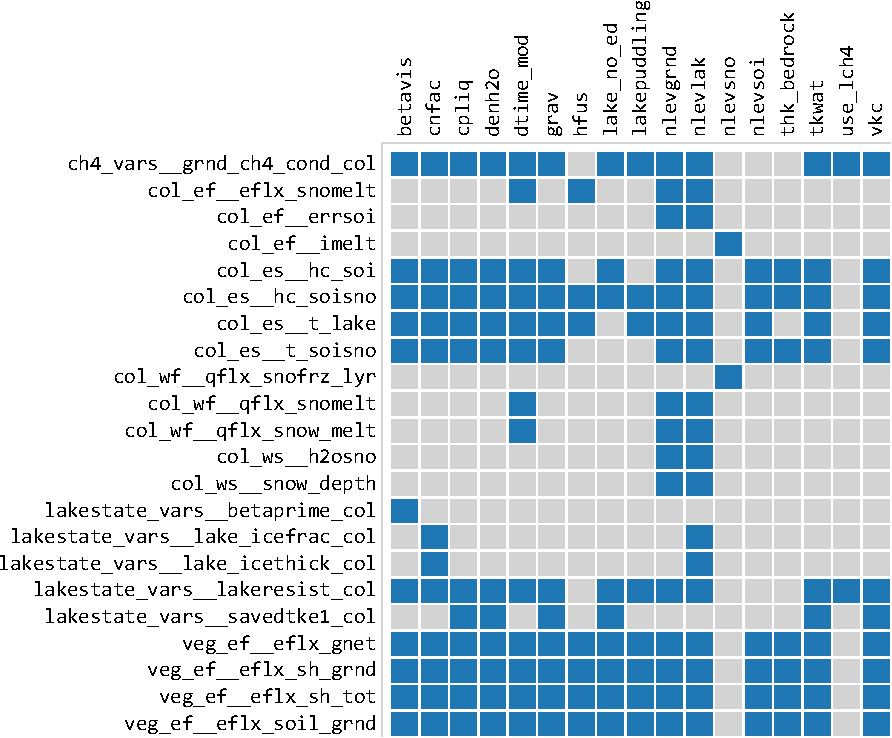
\includegraphics[width=0.9\linewidth]{figures/change_impact_table.pdf}
    \caption{A mapping of the model constants (columns) and the model outputs (rows) they affect}
    \label{fig:changed_outputs}
\end{figure}

Finally, we used a third plugin, NetCDF4 Output, to combine output data and samples from
each sample group into a compressed NetCDF file. This allowed us to graph relationships 
between model constants and model outputs, an example of which can be seen in 
\Cref{fig:example_graph}.

\begin{figure}[ht]
    \centering
    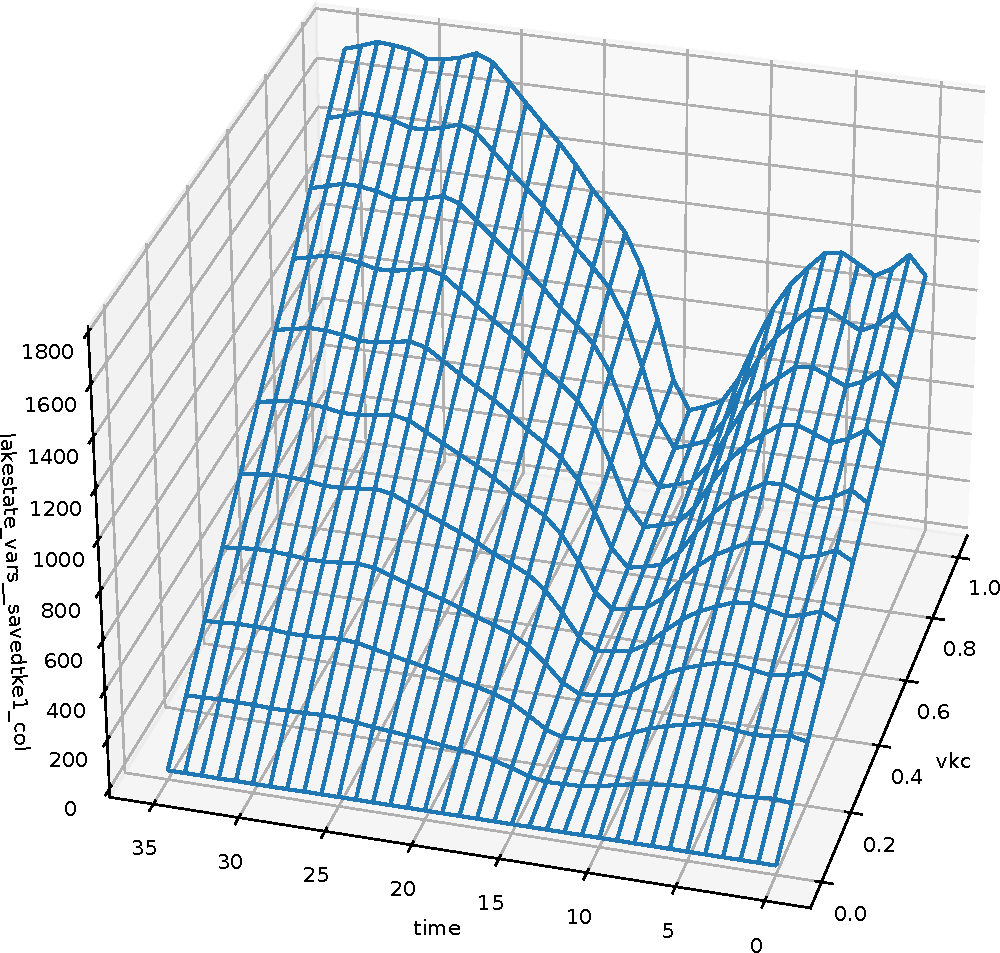
\includegraphics[width=0.9\linewidth]{figures/change_impact.pdf}
    \caption{
        \texttt{saved\_tke1\_col} changing in response to a 
        change in \texttt{vkc}, a model constant
    }
    \label{fig:example_graph}
\end{figure}

%\pagebreak
\subsection{
    \texorpdfstring{\raggedright Combinatorial and Property-Based \\ Testing}
    {Combinatorial and Property-Based Testing}
}

Our change-impact analysis demonstrated that many model outputs changed as a function of
multiple model constants. This motivated us to apply combinatorial testing because 
empirical data has shown that most software failures are caused by interactions between a 
small number of inputs \cite{combinatorial-emperical}. Additionally, we did not have a
test oracle for \verb|LakeTemperature|, but we did know that its outputs should be  
consistent with physical laws and boundaries, which led us to apply property-based 
testing. 

We used NIST's Advanced Combinatorial Testing System (ACTS) \cite{acts} to generate our 
test cases. Since
most of the model constants for \verb|LakeTemperature| are floating-point, which
ACTS doesn't support,  
we separated the generation of test cases in
ACTS from the process of mapping those to actual values. We added each model 
constant as an integer variable in ACTS and asked it to use the values in $\{0, 1, \dots, 
n - 1\}$, where $n$ is the number of values we wanted to test for that 
constant. We mapped those indices to values we manually defined in a NetCDF 
\term{partition file}, from which we made a compressed NetCDF file containing 
the completed test cases. This file was then used by our NetCDF Cases plugin. An 
example of this process is shown in \Cref{lst:example_acts_mapping}.

\begin{lstlisting}[
    caption=Example NetCDF test cases created from an ACTS CSV file,
    language=justcomment,
    float,
    floatplacement=ht,
    label=lst:example_acts_mapping
]
# Example ACTS CSV
var_1,var_2
0,0
0,1
1,0
1,1
2,0
2,1

# Example NetCDF Partition
var_1 = 0.1, 0.5, 0.9 ;
var_2 = 15, 18 ;

# Example NetCDF Cases
var_1 = 0.1, 0.1, 0.5, 0.5, 0.9, 0.9 ;
var_2 = 15, 18, 15, 18, 15, 18 ;
\end{lstlisting}

Typically with combinatorial testing, all legal values for the input parameters are
used. This is feasible for boolean and integer values, but the number of possible 
floating-point values, even a small range, is far too many to test. Experiments
have shown that even and random partitioning of a continuous domain is less effective than 
partitioning based on values known by the developers of the software
\cite{combinatorial-continuous}. The domain scientists at Oak Ridge National Laboratory 
(ORNL) provided us with extreme bounds and default values that could exercise different 
branches in \verb|LakeTemperature|, some of which are shown in \Cref{tab:constant_ranges}
\cite{peter-and-dali}. We linearly interpolated these ranges for both integer and floating-
point constants in order to test values between these extremes.

\begin{table}[ht]
    \centering
    \caption{
        An example of extreme ranges and defaults for model constants provided by domain 
        scientists
    }
    \label{tab:constant_ranges}
    \begin{tabular}{c c c c}
        \toprule
        Constant & Default & Lower & Upper \\
        \midrule
        \verb|betavis| & 0.0 & 0.0 & 1.0 \\
        \verb|cnfac| & 0.5 & 0.0 & 1.0 \\
        \verb|nlevlak| & 10 & 2 & 25 \\
        \verb|grav| & 9.806 & 9.700 & 9.860 \\
        \bottomrule
    \end{tabular}
\end{table}

For property-based testing, we needed to define properties we expected model 
outputs to follow. We wrote the Fault Finding plugin to 
implement \term{checks}, small functions that request only specific model constants 
and model outputs needed to verify a property. Each check results in a status inspired by unit test frameworks, where 
``pass'' means the function is run without error, and ``fail'' means an assertion fails. We 
also added the ``error'' status for when an error is thrown, and a ``skipped'' status for when 
a precondition for the check is not met.

We wrote our checks based on documentation provided by domain scientists at ORNL that 
included boundaries for model outputs, aggregation rules, and scenarios we could use to 
test key physical laws \cite{peter-and-dali}. Since our framework was not designed to test 
specific scenarios, we implemented those as conditional checks, which first checked to see 
if their scenarios matched any of the columns in the output, and would return a 
``skipped'' status if none did. An example can be viewed in \Cref{lst:example_check}.

\begin{lstlisting}[
    language=python,
    float,
    floatplacement=ht,
    caption=An example check for use with the Fault Finding plugin,
    label=lst:example_check
]
def check_methane_conductance_gated_by_ice(
  use_lch4,
  test_lakestate_vars_lake_icefrac_col,
  test_ch4_vars_grnd_ch4_cond_col,
):
  some_surface_ice = (
    test_lakestate_vars_lake_icefrac_col[
      :, 0, :
    ] > 0.1
  )

  if (
    not use_lch4 == 1
    or not np.any(some_surface_ice)
  ):
    return CheckStatus.SKIPPED

  conducting_methane = (
    test_ch4_vars_grnd_ch4_cond_col > 0.0
  )

  # Verify methane blocked by ice
  assert not np.any(
    some_surface_ice & conducting_methane
  )
\end{lstlisting}

\section{Experimental Results}
\label{sec:results}

% Can include tables for test case generation and runtime.
% Discuss that all checks were either passed or skipped when we interpolated between
% bounds, describe why each skipped check was skipped.
% Discuss the implications of our results, even if we didn't find any bugs.

We limited \verb|LakeTemperature|'s time steps to 35 in order to reduce
the amount of time it took to run \verb|elmtest.exe|. With this configuration, we found
that it took \verb|elmtest.exe| an average of 0.456 seconds to run on our machine, with a 
standard deviation of 0.040 seconds and a sample size of ten runs. (Time was measured 
using ``real'' time from the shell keyword \verb|time| in Bash.) We were able to run cases 
with a degree of interaction (DoI) of 2--4. Additionally, while we tested 17 constants in
our change-impact analysis, we only tested 15 in our combinatorial cases. This is because
we decided to keep \verb|nlevsoi| and \verb|nlevsno| at their defaults since \verb|nlevsoi|'s 
range was given in terms of other constants, which isn't supported by our current testing 
model, and we discovered increasing \verb|nlevsno| beyond its default of five resulted in 
a $-6$ exit code, causing over 90\% of our cases to crash. Simple statistics about running 
these test cases are given in \Cref{tab:test_time}. Note that ``crashed cases'' refer to 
cases where \verb|elmtest.exe| returned a nonzero exit code, in our testing, either $-6$ or 
$-11$.

\begin{table}[ht]
    {
        \centering
        \caption{Time taken to run test suites and number of cases}
        \label{tab:test_time}
        \begin{tabular}{c c c c}
            \toprule
            DoI & \# of Cases & Run Time & \# of Crashes \\
            \midrule
            2 & 122 & 00:00:55 & 21 \\
            3 & 3,516 & 00:26:37 & 611 \\
            4 & 50,031 & 07:58:36$^*$ & 9,563 \\
            \bottomrule
        \end{tabular} \\
    }
    \vspace{6pt}
    \footnotesize
    $^*$This suite was run on a slower machine. The average time to run \verb|elmtest.exe|
    was used to estimate the time on the primary machine.
\end{table}

We had 40 checks in total, 22 of which passed on every case and an additional 5 skipped 
at least one case but never failed (only one of which skipped every case). We had 13 checks
fail at least once, the status counts of which are given in \Cref{tab:check_statuses}.

\begin{table*}[tb]
    \centering
    \caption{Status counts for each check, per test suite (passed/skipped/failed)}
    \label{tab:check_statuses}
    \footnotesize
    \begin{tabular}{l c c c}
    \toprule
    Check & DoI: 2 & DoI: 3 & DoI: 4 \\
    \midrule
    \verb|combined_heat_content_not_less_than_soil_heat_content|
    & 4/0/97 & 121/0/2,784 & 1,644/0/38,824 \\
    \verb|errsoi_almost_zero|
    & 4/0/97 & 121/0/2,784 & 1,644/0/38,824 \\
    \verb|ground_methane_conductance_finite|
    & 71/0/30 & 2,031/0/874 & 28,339/0/12,129 \\
    \verb|icethick_col_is_sum|
    & 40/0/61 & 1,176/0/1,729 & 16,244/0/24,224 \\
    \verb|lake_temperature_finite|
    & 4/0/97 & 121/0/2,784 & 1,644/0/38,824 \\
    \verb|lake_transport_resistance_finite|
    & 71/0/30 & 2,031/0/874 & 28,339/0/12,129 \\
    \verb|lake_water_transport_resistance_not_negative|
    & 71/0/30 & 2,031/0/874 & 28,339/0/12,129 \\
    \verb|latent_heat_from_lake|
    & 27/73/1 & 850/2,037/18 & 16,267/22,102/2,099 \\
    \verb|melting_latent_heat|
    & 0/101/0 & 0/2,905/0 & 0/40,457/11 \\
    \verb|methane_conductance_non_negative|
    & 20/51/30 & 587/1,444/874 & 8,160/20,179/12,129 \\
    \verb|soil_heat_content_not_negative|
    & 4/0/97 & 121/0/2,784 & 1,644/0/38,824 \\
    \verb|soil_snow_temperature_finite|
    & 4/0/97 & 121/0/2,784 & 1,644/0/38,824 \\
    \verb|temp_at_freezing_where_lake_is_frozen|
    & 28/73/0 & 852/2,037/16 & 16,284/22,102/2,082 \\
    \bottomrule
\end{tabular} \\
\end{table*}

% Note from Aidan:
% Here's what we had here originally (before the results changed). We made explainations for
% why checks skipped. We can't really do that for why our checks failed since we haven't had
% time to investigate, but I wanted to acknowledge that in this comment.

%The checks that were skipped entirely depended on having a lake with a frozen surface,
%which did not occur within the 35 time steps. Additionally, the checks that were skipped
%half of the time pertained to methane conductance, and were skipped when this behavior
%was disabled (\verb|use_lch4 = false|).
%
%While our testing ultimately did not reveal any faults in \verb|LakeTemperature|, we 
%believe it demonstrated the usefulness and adaptability of our functional testing 
%framework, and that it could be used for stronger testing of this subroutine and other
%subroutines of ELM in the future.

Our results from combinatorial and property-based testing are preliminary. 
We are investigating the reasons for the failed checks. It could be due to  
our implementation of them, SPEL, or \verb|LakeTemperature|. Currently, many of them seem to have failed due to receiving NaN values, possibly
suggesting some combinations of constants are invalid. While our results are limited, we 
believe they demonstrate the usefulness and adaptability of our functional testing 
framework, and its ability to be used for more rigorous testing of this subroutine and other
subroutines of ELM in the future.

\section{Conclusion and Future Work}
\label{sec:conclusion}

We proposed an automated functional testing framework for ELM subroutines that supports 
different methods of input space reduction and solutions to the test oracle problem using
plugins. We demonstrated the use of our framework by performing change-impact analysis as 
well as combinatorial and property-based testing on \verb|LakeTemperature|.

One limitation of our testing framework is that it currently only supports modification of 
the model constants. We can control physical and numerical constants this way, but without
controlling model inputs, we cannot modify the simulation's starting data. For this 
reason, we were unable to fully test the scenarios provided to us by domain scientists and 
had to make them conditional checks instead.

Our testing results are preliminary. We are in the process of analyzing what
combinations of constants cause \verb|elmtest.exe| to crash, as well as determining wether our
failing checks represent a flaw in our test design or a bug in either SPEL or \verb|LakeTemperature|.

Given the extensibility of our framework, there are many ways our work can be expanded on 
in the future. Firstly, adding the ability for our framework to modify model inputs would
allow us to test specific scenarios. Additionally, we could parallelize our testing 
framework, since samples are run independently. We could implement more testing methods
using sampling plugins, such as statistical testing. Finally, as \verb|SPEL| supports more 
subroutines of ELM, we can apply our framework to those.

\section*{Acknowledgments}

% Note from Aidan:
% I know we cut this disclaimer for space, but are we sure it's not required by the NSF?

This work was generously funded by the National Science Foundation (NSF) as part of NSF
Grant 2209834. %Any opinions, findings, conclusions, or recommendations expressed in
%this material are those of the authors and do not necessarily reflect the views of the 
%NSF.

\bibliographystyle{latex8}
\bibliography{paper.bib}

\end{document}
